\documentclass[pdf]{beamer}
\mode<presentation>{}

\newcommand{\G}{\textcolor{blue}{G}}
\newcommand{\n}{\textcolor{red}{n}}
\newcommand{\V}{\textcolor{teal}{V}}
\newcommand{\E}{\textcolor{olive}{E}}
\newcommand{\T}{\textcolor{orange}{T}}

\usepackage{color,tikz}
\usefonttheme{serif}

%% preamble
\title{Ore's Theorem}
\subtitle{CS 111 Presentation}
\author{Youssef Adam \and Thomas Kang \\ Youssef Koreatam \and Michael Wong \and Gabriel Serrano}
\date{March 19, 2024}
\institute{Department of Computer Science, University of California, Riverside}
\begin{document}

    %% title frame
    \begin{frame}
        \titlepage
    \end{frame}

    %% questions
    \begin{frame}{Questions}

    \end{frame}

    %% introduction frame
    \begin{frame}{Introduction: Background Knowledge}
        To understand \textbf{Ore's theorem}, we must briefly recapitulate
        what it means for a graph to be \textbf{Hamiltonian}.
        \pause
        \vspace{10px}
        \\Let $\G(\V,\E)$ be an undirected graph with $|\V| \geq 3$ vertices. \pause
        \\If we are able to create a cycle $\T$ that meets each and every
        vertex strictly once, then $\G$ is considered \textbf{Hamiltonian}.
        \pause
        \vspace{20px}
        \\\textcolor{cyan}{\underline{Example:}}
        \vspace{10px}
        \begin{figure}
            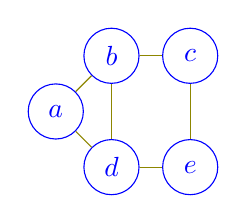
\begin{tikzpicture}[auto,node distance=1cm,scale=1, main/.style = {minimum size=0.7cm, color=blue, draw, circle},
                every path/.style = {color=olive}]
                \node[main] (1) {$a$};
                \node[main] (2) [above right of=1] {$b$};
                \node[main] (3) [right of=2] {$c$};
                \node[main] (4) [below right of=1] {$d$};
                \node[main] (5) [right of=4] {$e$};
                \path[every node/.style={font=\sffamily\small}]
                    (1) edge node [right] {} (2)
                    (1) edge node [right] {} (4)
                    (2) edge node [right] {} (4)
                    (2) edge node [right] {} (3)
                    (4) edge node [right] {} (5)
                    (3) edge node [right] {} (5);
            \end{tikzpicture}
            \pause
            \hspace{50px}
            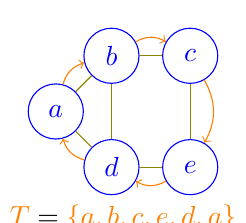
\begin{tikzpicture}[auto,node distance=1cm,scale=1, main/.style = {minimum size=0.7cm, color=blue, draw, circle}]
                \node[main] (1) {$a$};
                \node[main] (2) [above right of=1] {$b$};
                \node[main] (3) [right of=2] {$c$};
                \node[main] (4) [below right of=1] {$d$};
                \node[main] (5) [right of=4] {$e$};
                % \draw (1) -- (2); \draw (1) -- (3); \draw (2) -- (4);
                % \draw (3) -- (4); \draw (4) -- (5); \draw (5) -- (6); \draw (4) -- (6);
                \path[every node/.style={font=\sffamily\small},{color=olive}]
                    (1) edge node [right] {} (2)
                    (1) edge node [right] {} (4)
                    (2) edge node [right] {} (4)
                    (2) edge node [right] {} (3)
                    (4) edge node [right] {} (5)
                    (3) edge node [right] {} (5);
                \path[->,every node/.style={font=\sffamily\small},{color=orange}]
                    (1) edge[bend left] node [left] {} (2)
                    (2) edge[bend left] node [left] {} (3)
                    (3) edge[bend left] node [left] {} (5)
                    (5) edge[bend left] node [left] {} (4)
                    (4) edge[bend left] node [left] {} (1);
                %     (6) edge[bend right] node [left] {} (5)
                %     (5) edge[bend right] node [left] {} (4);
                \node[overlay, anchor=north] at (current bounding box.south) {$\T = \textcolor{orange}{\{a, b, c, e, d, a\}}$};
            \end{tikzpicture}
        \end{figure}
    \end{frame}
    %% Declare Ore's theorem formally in this slide.
    %% During the video presentation, we will break it down into informal parts
    %% so as to make presenting easier (and longer--remember we have to talk for
    %% at least 7 minutes!)
    \begin{frame}{Introduction: Ore's Theorem Statement}

    \end{frame}

    %% Create an example of Ore's theorem and go through it.
    \begin{frame}{Examples}

    \end{frame}

    %% Create a second examples of Ore's theorem.
    \begin{frame}{Examples}

    \end{frame}

    %% (OPTIONAL) Create a third example of Ore's theorem.
    \begin{frame}{Examples}

    \end{frame}

    %% Describe the applications of graph theory and relate that to Hamiltonian
    %% paths and the importance of efficiency in finding them. This can be as
    %% many slides as you want.
    \begin{frame}{Applications}

    \end{frame}

    %% Summarize everything this presentation has covered, from the statement of Ore's Theorem to its Applications.
    \begin{frame}{Conclusion: Summary}

    \end{frame}

    %% Restate the questions.
    \begin{frame}{Conclusion: Questions}

    \end{frame}

\end{document}